\documentclass[11pt,a4paper]{article}
\usepackage[utf8]{inputenc}
\usepackage[T1]{fontenc}
\usepackage{mathptmx}
\usepackage[margin=2.5cm]{geometry}
\usepackage{amsmath,amssymb}
\usepackage{booktabs,array,tabularx,multirow}
\usepackage{enumitem}
\usepackage{setspace}
\usepackage{fancyhdr}
\usepackage{graphicx}
\usepackage{tikz}
\usetikzlibrary{arrows.meta,positioning}
\usepackage{pgfplots}
\pgfplotsset{compat=1.17}
\usepackage[colorlinks=true,linkcolor=black,citecolor=black,urlcolor=black]{hyperref}

\setstretch{1.0}
\setlength{\parindent}{1.2em}
\setlength{\parskip}{2pt}
\setlist{itemsep=1pt,topsep=3pt}
\renewcommand{\arraystretch}{1.12}
\pagestyle{fancy}
\fancyhf{}
\fancyhead[L]{\small Práctica Investigativa III, 2026-2 -- Informe 3: Resultados y discusión}
\fancyfoot[C]{\small\thepage}
\renewcommand{\headrulewidth}{0.3pt}
\emergencystretch=2em

\renewcommand{\abstractname}{Resumen}
\renewcommand{\refname}{Referencias}
\renewcommand{\tablename}{Tabla}
\renewcommand{\figurename}{Figura}
\renewcommand{\appendixname}{Apéndice}

\newcommand{\gr}{$^{\circ}$}
\newcommand{\Mae}{\mathrm{MAE}}
\newcommand{\R}{\mathbb{R}}
\newcommand{\E}{\mathbb{E}}

\begin{document}

\noindent\fbox{\parbox{\dimexpr\textwidth-2\fboxsep-2\fboxrule\relax}{%
\small\textbf{Visto bueno del tutor científico} (Juan David Martínez Vargas, Universidad EAFIT)\\[10pt]
Firma: \hrulefill\hspace{1.5em} Fecha: \rule{3cm}{0.4pt}}}

\vspace{10pt}
\begin{center}
{\large\bfseries Resultados y discusión de un autoencoder recurrente de ciclos de marcha:\\ cierre del ciclo, eliminación de ruido y codificador fundacional congelado}\\[8pt]
Jesús David Cantellón\\
{\small Universidad EAFIT, Práctica Investigativa III (2026-2)}\\
{\small Profesor de la asignatura: Fredy Hernán Marín Sánchez \quad|\quad Tutor científico: Juan David Martínez Vargas}\\
{\small 8 de noviembre de 2026}
\end{center}

\begin{abstract}\noindent
\textit{Introducción.} Un autoencoder recurrente (GRU) de ciclos de marcha de seis ángulos articulares en 101 puntos tuvo, en la comparación inicial del proyecto NeuroStrideAI, el mayor error de reconstrucción entre los modelos que aprenden de los datos y ciclos reconstruidos cuyos extremos no coinciden. \textit{Métodos.} Se evaluaron dos modificaciones (código latente en cada paso del decodificador y pérdida de cierre del ciclo) en la variante con ciclos limpios (A) y en la entrenada con ciclos dañados (B), con cinco semillas, partición por sujeto (240 ciclos de entrenamiento) y prueba t pareada; se evaluaron también ensambles, regularizaciones adicionales y un codificador fundacional de series de tiempo congelado (TimesFM 2.5) con dos controles. \textit{Resultados.} En A, el error absoluto medio bajó de 4.99\gr{} a 4.11\gr{} y el salto entre el primer y el último punto de 5.07\gr{} a 0.87\gr{}; en B, el salto bajó de 3.04\gr{} a 0.57\gr{} y la ganancia de corrección subió de 0.296 a 0.337. El codificador fundacional tuvo un error de 7.19\gr{}, igual al de pesos aleatorios ($p=0.83$) y mayor que el del GRU, y una proyección lineal de la serie cruda tuvo un error menor (3.69\gr) que el GRU. \textit{Discusión.} Los resultados son coherentes con un límite impuesto por el tamaño de los datos y con la competitividad de modelos lineales con pocas muestras. \textit{Conclusión.} Las dos modificaciones mejoran la fidelidad y el cierre; el modelo fundacional congelado, en este diseño, no aporta. Se discuten las limitaciones, entre ellas la selección de hiperparámetros sobre el conjunto de prueba de control.
\end{abstract}

\noindent\textbf{Palabras clave:} análisis de marcha, autoencoder, red recurrente, cierre de ciclo, modelo fundacional de series de tiempo.

%====================================================================
\section{Introducción}
\label{sec:intro}

El proyecto NeuroStrideAI (exoesqueleto pediátrico) busca un modelo normativo de ciclos completos de marcha. Cada ciclo estandarizado se trata como $G\in\R^{101\times 6}$ (101 instantes y seis ángulos articulares) y se modela con un autoencoder $f=D_\psi\circ E_\phi$ que comprime $G$ en un código $z\in\R^d$ y lo reconstruye \cite{hinton2006}. En la comparación inicial del proyecto \cite{neurostride2026}, el autoencoder recurrente tuvo el mayor error de reconstrucción entre los modelos que aprenden de los datos (5.17\gr{} y 5.35\gr) y reconstruyó ciclos cuyos extremos no coinciden (saltos de 4.94\gr{} y 3.45\gr), aunque la marcha es periódica; un modelo lineal (PCA) tuvo un error de 2.78\gr. El Informe 1 identificó esta incoherencia y tres vacíos de la literatura revisada: la reconstrucción periódica de ciclos completos (V1), la evaluación conjunta de fidelidad, corrección y forma (V2) y el uso de modelos fundacionales congelados como codificadores de ciclos de marcha (V3).

Este informe presenta los resultados y la discusión de las cinco hipótesis formuladas en el Informe 1 y descritas en los métodos del Informe 2. Sean $\mathcal E$ el error absoluto medio de reconstrucción, $\mathcal J$ el defecto de cierre (diferencia media entre el primer y el último punto del ciclo reconstruido) y $\gamma$ la ganancia de corrección, todos definidos en la sección~\ref{sec:metricas}.

\begin{table}[h]
\centering\footnotesize
\begin{tabularx}{\textwidth}{@{}l>{\raggedright\arraybackslash}X>{\raggedright\arraybackslash}p{2.6cm}@{}}
\toprule
Hipótesis & Enunciado & Se contrasta en \\
\midrule
H1 & Entregar $z$ en cada paso del decodificador reduce $\mathcal E$. & Sección~\ref{sec:r2} \\
H2 & La pérdida de cierre reduce $\mathcal J$ y existe un peso $w^\ast$ con $\mathcal E(f_{w^\ast})-\mathcal E(f_0)\le\varepsilon$, con $\varepsilon=0.23$\gr{}, una desviación estándar entre semillas del error del modelo original. & Secciones~\ref{sec:r2} y~\ref{sec:r4} \\
H3 & Las dos modificaciones, en la variante con eliminación de ruido, reducen $\mathcal J$ y aumentan $\gamma$. & Sección~\ref{sec:r3} \\
H4 & Un ensamble de cinco modelos reduce $\mathcal E$ y $\mathcal J$ frente al promedio de sus miembros. & Sección~\ref{sec:r5} \\
H5 & Un codificador fundacional congelado mejora $\mathcal E$ o $\gamma$ frente al autoencoder recurrente mejorado. & Secciones~\ref{sec:r8} y~\ref{sec:r9} \\
\bottomrule
\end{tabularx}
\caption{Hipótesis contrastadas en este informe.}
\label{tab:hip}
\end{table}

%====================================================================
\section{Métodos}
\label{sec:metodos}

Esta sección resume los métodos descritos en el Informe 2, de modo que el informe sea autocontenido.

\subsection{Datos y partición}
\label{sec:datos}

Los ciclos proceden del procedimiento del proyecto: video de marcha, estimación de pose \cite{fang2023alphapose}, ángulos sagitales de cadera, rodilla y tobillo de ambas piernas a 30 Hz, interpolación a 101 puntos con PCHIP \cite{fritsch1980} y un control de calidad (15 a 90 cuadros, al menos 90\% de valores finitos, salto máximo entre cuadros de 17\gr{} y diferencia entre el primer y el último valor no mayor de 25\gr). De 551 intervalos originales quedaron 461 ciclos válidos de 64 personas. La partición es por sujeto \cite{saeb2017}: los controles se dividen (semilla 42) en 70\%, 15\% y 15\%, y los casos (niños con parálisis cerebral) forman un conjunto de prueba externo que nunca interviene en el ajuste (tabla~\ref{tab:particion}). Cada señal se estandariza con la media y la desviación estándar del conjunto de entrenamiento; las métricas en grados se calculan tras invertir la estandarización.

\begin{table}[h]
\centering\small
\begin{tabular}{llcc}
\toprule
Conjunto & Grupo & Sujetos & Ciclos \\
\midrule
Entrenamiento & control & 28 & 240 \\
Validación & control & 6 & 44 \\
Prueba de control & control & 7 & 47 \\
Prueba externa & casos & 23 & 130 \\
\midrule
Total & & 64 & 461 \\
\bottomrule
\end{tabular}
\caption{Partición por sujeto.}
\label{tab:particion}
\end{table}

\subsection{Modelos}
\label{sec:modelos}

\textbf{Autoencoder recurrente base.} El codificador es una GRU \cite{cho2014} bidireccional \cite{schuster1997} de 48 unidades por dirección cuyo estado final produce $z=W_e[\overrightarrow h_{101};\overleftarrow h_1]+b_e\in\R^d$. El decodificador es una GRU de 48 unidades con estado inicial $h_0=W_0z+b_0$ y entrada $u_t=[\sin2\pi\tau_t,\cos2\pi\tau_t]$, con $\tau_t=(t-1)/100$, y salida $\hat g_t=W_oh_t+b_o$. Se entrena con ciclos limpios (modelo A) o con ciclos dañados como entrada y limpios como objetivo (modelo B, sección~\ref{sec:dano}).

\textbf{Modificación 1.} El código se concatena a la entrada del decodificador en los 101 pasos, $u_t'=[\sin2\pi\tau_t,\cos2\pi\tau_t,z]$.

\textbf{Modificación 2.} Se añade a la pérdida un término de cierre con peso $w\ge0$:
\begin{equation}
\mathcal L=\frac{1}{606}\sum_{t=1}^{101}\sum_{c=1}^{6}(\hat g_{t,c}-g_{t,c})^2+w\cdot\frac16\sum_{c=1}^{6}\left|\hat g_{1,c}-\hat g_{101,c}\right| .
\end{equation}
Las configuraciones finales son $d=32$ y $w=0.1$ (A) y $d=16$ y $w=0.05$ (B). El modelo original reproducido usa $d=16$, $w=0$ y el código solo en el estado inicial. Un ensamble promedia las predicciones de cinco modelos con semillas distintas \cite{dietterich2000}.

\subsection{Daño sintético para la variante con eliminación de ruido}
\label{sec:dano}

Para cada canal $c$ se genera $\tilde g_{t,c}=m_c+a_c(g_{t,c}-m_c)+b_c+\varepsilon_{t,c}$, con $m_c$ la media del canal, $a_c\sim U(0.5,1.8)$, $b_c\sim U(-0.9,0.9)$ y $\varepsilon_{t,c}\sim\mathcal N(0,0.15^2)$, seguido de un desplazamiento circular entero $s\sim U\{-8,\dots,8\}$ por pierna \cite{vincent2008}. La validación y la parada temprana usan ciclos limpios.

\subsection{Componentes adicionales, codificador fundacional y controles}
\label{sec:fm_met}

Se exploraron regularizaciones sobre las diferencias consecutivas con índices circulares $\Delta g_t=g_{t+1}-g_t$ (suavidad, curvatura, igualar incrementos, igualar pendientes en la costura, núcleo periódico y ponderación por fase), cambios de arquitectura (decodificador bidireccional, atención \cite{bahdanau2015}, velocidad angular y asimetría como entradas) y cambios de entrenamiento del modelo B (consistencia de códigos, intensidad y currículo del daño).

El codificador fundacional es TimesFM 2.5 \cite{das2024timesfm,timesfm25}, congelado. Cada señal estandarizada se remuestrea a 128 puntos (cuatro parches de 32); se toma el estado oculto del bloque de índice 9 (el décimo), se promedian los parches, se añade el estado del último parche y la media y la desviación estándar de la serie (2562 características por canal, 15\,372 en total) y una capa lineal entrenable las proyecta a $z$. El decodificador es el mejorado. El bloque, la agrupación y el decaimiento de pesos se eligieron entre ocho configuraciones con el conjunto de validación y una semilla (apéndice~\ref{app:timesfm}). Se usan dos controles con el mismo decodificador y las mismas semillas: TimesFM con pesos aleatorios (con las escalas de las normas internas fijadas en uno) y una proyección lineal de la serie cruda aplanada (606 valores). Una primera versión del control aleatorio usó la inicialización por defecto, en la que las escalas de las normas valen cero y los bloques actúan como identidad; se corrigió y se repitió (sección~\ref{sec:r8}).

\begin{figure}[h]
\centering
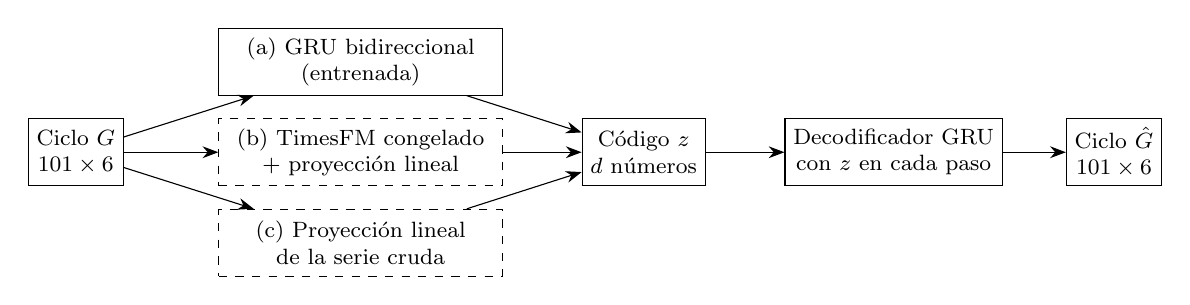
\begin{tikzpicture}[
 box/.style={draw,rectangle,minimum height=0.85cm,align=center,font=\footnotesize,inner sep=3pt},
 arr/.style={-{Stealth[length=2mm]}}]
\node[box] (in) {Ciclo $G$\\ $101\times 6$};
\node[box,right=1.2cm of in,yshift=1.15cm,minimum width=3.6cm] (e1) {(a) GRU bidireccional\\ (entrenada)};
\node[box,right=1.2cm of in,minimum width=3.6cm,dashed] (e2) {(b) TimesFM congelado\\ + proyección lineal};
\node[box,right=1.2cm of in,yshift=-1.15cm,minimum width=3.6cm,dashed] (e3) {(c) Proyección lineal\\ de la serie cruda};
\node[box,right=1.0cm of e2] (z) {Código $z$\\ $d$ números};
\node[box,right=1.0cm of z,minimum width=2.4cm] (dec) {Decodificador GRU\\ con $z$ en cada paso};
\node[box,right=0.8cm of dec] (out) {Ciclo $\hat G$\\ $101\times 6$};
\draw[arr] (in) -- (e1); \draw[arr] (in) -- (e2); \draw[arr] (in) -- (e3);
\draw[arr] (e1) -- (z); \draw[arr] (e2) -- (z); \draw[arr] (e3) -- (z);
\draw[arr] (z) -- (dec); \draw[arr] (dec) -- (out);
\end{tikzpicture}
\caption{Esquema del autoencoder. Un mismo decodificador se compara con tres codificadores: (a) GRU de los modelos A y B, (b) TimesFM congelado con proyección lineal entrenable y (c) proyección lineal de la serie cruda (control). Las líneas discontinuas indican las alternativas de las secciones~\ref{sec:r8} y~\ref{sec:r9}.}
\label{fig:esquema}
\end{figure}

\subsection{Protocolo, métricas y análisis estadístico}
\label{sec:metricas}

Las redes se implementan en PyTorch \cite{paszke2019} y se entrenan con Adam \cite{kingma2015} (tasa $10^{-3}$, lotes de 64, hasta 100 épocas, recorte de gradiente a 1.0 \cite{pascanu2013}, parada temprana con paciencia de 12 \cite{prechelt1998}). Los modelos GRU se ejecutaron en CPU y los que usan TimesFM, en GPU. Cada configuración se entrena con cinco semillas (42, 1, 7, 123 y 2024). Las métricas, en grados, son las siguientes, con $N$ el número de ciclos del conjunto:
\begin{align}
\mathcal E&=\Mae=\frac{1}{606N}\sum_{n}\sum_{t,c}\left|\hat g^{(n)}_{t,c}-g^{(n)}_{t,c}\right|,\qquad
\mathcal J=\frac{1}{6N}\sum_{n}\sum_{c}\left|\hat g^{(n)}_{1,c}-\hat g^{(n)}_{101,c}\right|,\\
\gamma&=1-\frac{\Mae(f(\tilde G),G)}{\Mae(\tilde G,G)},
\end{align}
evaluadas en 47 ciclos limpios de prueba de control ($\mathcal E$, $\mathcal J$) y en los mismos ciclos dañados con una realización fija (semilla 42) del daño ($\gamma$). Sobre los 130 ciclos de casos externos se calculan la ganancia de tipicidad, $\frac1N\sum_n\big(1-d(f(x^{(n)}))/d(x^{(n)})\big)$ con $d$ la distancia al ciclo de control de entrenamiento más cercano, y la intervención, $\frac{1}{606N}\sum_n\sum_{t,c}|f(x^{(n)})_{t,c}-x^{(n)}_{t,c}|$, que no tiene sentido de ``mejor''. Las métricas de forma son la pendiente en la costura, $|(\hat g_2-\hat g_1)-(\hat g_{101}-\hat g_{100})|$, el error en incrementos, $\overline{|\Delta\hat g-\Delta g|}$, y la rugosidad, $\overline{|\Delta^2\hat g|}$.

Para cada métrica y semilla $s$ se calcula la diferencia pareada entre configuración y referencia; con media $\bar\Delta$ y desviación $s_\Delta$ de las cinco diferencias, el estadístico $T=\bar\Delta/(s_\Delta/\sqrt5)\sim t_4$ bajo la hipótesis nula de diferencia media cero, y el intervalo de confianza de 95\% es $\bar\Delta\pm2.776\,s_\Delta/\sqrt5$. La prueba es de dos colas con $\alpha=0.05$, sin corrección por comparaciones múltiples. Los resultados con una semilla son exploratorios y no se usan como evidencia.

%====================================================================
\section{Resultados}
\label{sec:resultados}

Cada resultado se numera (R1 a R10), indica la sección de métodos que lo origina y la hipótesis que contrasta. Las cifras son medias $\pm$ desviación estándar de cinco semillas, salvo que se indique otra cosa; los ensambles provienen de un único conjunto de cinco modelos. Los archivos de salida están en el repositorio (sección de disponibilidad, al final del informe).

\subsection{R1. Punto de partida y reproducción de los modelos originales}
\label{sec:r1}

\textit{Métodos: secciones~\ref{sec:datos} y~\ref{sec:modelos}. Hipótesis: ninguna (línea base).} La tabla~\ref{tab:inicial} reproduce la comparación inicial del proyecto \cite{neurostride2026}, con una corrida por modelo. Entre los modelos que aprenden de los datos, A y B tienen el mayor error y saltos de cierre de 4.94\gr{} y 3.45\gr{}; PCA tiene el menor error (2.78\gr) y el autoencoder convolucional con eliminación de ruido la mayor ganancia de corrección (0.412).

\begin{table}[h]
\centering\small
\setlength{\tabcolsep}{4pt}
\begin{tabular}{lccccc}
\toprule
Modelo & $\mathcal E$ (\gr) & $\mathcal J$ (\gr) & $\gamma$ & Tipicidad & Interv. (\gr) \\
\midrule
Media de controles & 8.77 & 0.60 & $-0.121$ & 0.132 & 10.83 \\
PCA & 2.78 & 3.41 & 0.207 & 0.127 & 3.86 \\
Autoencoder convolucional & 3.30 & 3.11 & 0.252 & 0.182 & 4.83 \\
Autoencoder convolucional con eliminación de ruido & 4.07 & 1.88 & 0.412 & 0.376 & 5.98 \\
Proceso gaussiano periódico & 3.30 & 0.60 & 0.215 & 0.192 & 3.86 \\
Modelo A (GRU) & 5.17 & 4.94 & 0.152 & 0.349 & 8.12 \\
Modelo B (GRU con eliminación de ruido) & 5.35 & 3.45 & 0.280 & 0.385 & 7.89 \\
\bottomrule
\end{tabular}
\caption{Resultado R1: comparación inicial de siete modelos (una corrida por modelo). $\mathcal E$: error absoluto medio; $\mathcal J$: salto de cierre; $\gamma$: ganancia de corrección; Interv.: intervención. La media de controles no aprende de los datos y su salto bajo es trivial.}
\label{tab:inicial}
\end{table}

Al reproducir los modelos A y B con el protocolo de cinco semillas, con datos reconstruidos a partir de los archivos entregados, se obtuvieron errores de $4.99\pm0.23$\gr{} (A) y $5.25\pm0.10$\gr{} (B), cercanos a las cifras iniciales. La comparación de las secciones siguientes usa esta reproducción como referencia, porque aplica el mismo protocolo que los modelos modificados.

\subsection{R2. Modelo A: código en cada paso y pérdida de cierre}
\label{sec:r2}

\textit{Métodos: sección~\ref{sec:modelos}. Hipótesis: H1 y H2.} La tabla~\ref{tab:A} compara el modelo A original reproducido con el mejorado (código en cada paso, $d=32$, $w=0.1$). El error baja $0.88$\gr{} (de $4.99$ a $4.11$\gr, $-17.6\%$) y el salto de cierre baja $4.20$\gr{} (de $5.07$ a $0.87$\gr, $-82.9\%$); la dispersión del error entre semillas baja de $0.23$\gr{} a $0.05$\gr. La ganancia de corrección no cambia de forma significativa, la de tipicidad baja levemente y la intervención baja de $7.78$\gr{} a $6.14$\gr.

\begin{table}[h]
\centering\small
\setlength{\tabcolsep}{3pt}
\begin{tabular}{lccccc}
\toprule
Modelo A & $\mathcal E$ (\gr) & $\mathcal J$ (\gr) & $\gamma$ & Tipicidad & Interv. (\gr) \\
\midrule
Original reproducido & $4.99\pm0.23$ & $5.07\pm0.55$ & $0.208\pm0.018$ & $0.345\pm0.008$ & $7.78\pm0.13$ \\
Mejorado & $4.11\pm0.05$ & $0.87\pm0.11$ & $0.189\pm0.012$ & $0.326\pm0.007$ & $6.14\pm0.10$ \\
Diferencia (mejorado $-$ original) & $-0.88\pm0.29$ & $-4.20\pm0.67$ & $-0.019\pm0.022$ & $-0.018\pm0.016$ & $-1.64$ \\
Valor $p$ & 0.001 & $<0.001$ & 0.077 & 0.034 & $<0.001$ \\
\bottomrule
\end{tabular}
\caption{Resultado R2: modelo A original reproducido y mejorado. Media $\pm$ desviación estándar de cinco semillas; la diferencia se acompaña de la semiamplitud del intervalo de confianza de 95\%. Valor $p$ de la prueba t pareada.}
\label{tab:A}
\end{table}

\begin{figure}[h]
\centering
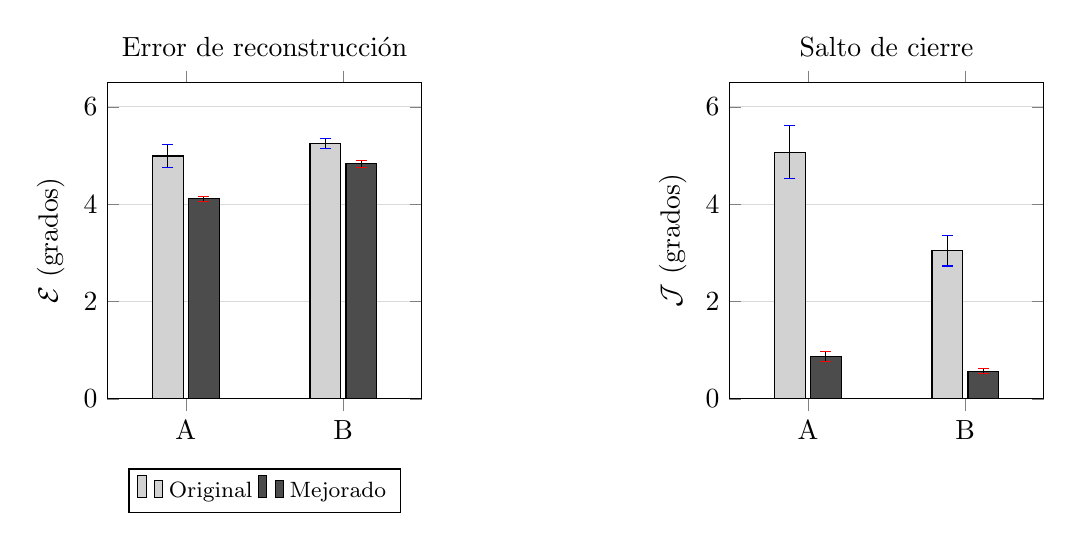
\begin{tikzpicture}
\begin{axis}[ybar,bar width=11pt,width=0.46\textwidth,height=5.6cm,ylabel={$\mathcal E$ (grados)},
 symbolic x coords={A,B},xtick=data,enlarge x limits=0.5,ymin=0,ymax=6.5,ymajorgrids,grid style={gray!30},
 title={Error de reconstrucción},error bars/y dir=both,error bars/y explicit,legend style={font=\footnotesize,at={(0.5,-0.22)},anchor=north,legend columns=-1}]
\addplot+[fill=gray!35,draw=black] coordinates {(A,4.99) +- (0,0.23) (B,5.25) +- (0,0.10)};
\addplot+[fill=black!70,draw=black] coordinates {(A,4.11) +- (0,0.05) (B,4.83) +- (0,0.07)};
\legend{Original,Mejorado}
\end{axis}
\begin{axis}[at={(7.9cm,0)},ybar,bar width=11pt,width=0.46\textwidth,height=5.6cm,ylabel={$\mathcal J$ (grados)},
 symbolic x coords={A,B},xtick=data,enlarge x limits=0.5,ymin=0,ymax=6.5,ymajorgrids,grid style={gray!30},
 title={Salto de cierre},error bars/y dir=both,error bars/y explicit]
\addplot+[fill=gray!35,draw=black] coordinates {(A,5.07) +- (0,0.55) (B,3.04) +- (0,0.31)};
\addplot+[fill=black!70,draw=black] coordinates {(A,0.87) +- (0,0.11) (B,0.57) +- (0,0.05)};
\end{axis}
\end{tikzpicture}
\caption{Resultados R2 y R3: error de reconstrucción $\mathcal E$ y salto de cierre $\mathcal J$ de los modelos A y B, original reproducido y mejorado. Las barras de error son una desviación estándar entre cinco semillas.}
\label{fig:barras}
\end{figure}

H2 se cumple en su primera parte (el cierre se reduce con $p<0.001$) y en la segunda, porque el error no solo no empeora respecto del original (bajo $\varepsilon=0.23$\gr), sino que baja. H1 se evalúa de forma aislada solo con una semilla (sección~\ref{sec:r4}); en la combinación se confirma la reducción del error.

\subsection{R3. Modelo B (eliminación de ruido): código en cada paso y pérdida de cierre}
\label{sec:r3}

\textit{Métodos: secciones~\ref{sec:modelos} y~\ref{sec:dano}. Hipótesis: H3.} Las mismas modificaciones mejoran el modelo B en las cinco semillas en las cuatro métricas principales (tabla~\ref{tab:B} y figura~\ref{fig:barras}). El error baja $0.42$\gr{} ($-8.0\%$), el salto baja $2.48$\gr{} ($-81.4\%$), la ganancia de corrección sube de $0.296$ a $0.337$ y la de tipicidad de $0.383$ a $0.414$, todos con $p\le0.002$. La mejora en corrección es modesta en términos absolutos. H3 se cumple.

\begin{table}[h]
\centering\small
\setlength{\tabcolsep}{3pt}
\begin{tabular}{lccccc}
\toprule
Modelo B & $\mathcal E$ (\gr) & $\mathcal J$ (\gr) & $\gamma$ & Tipicidad & Interv. (\gr) \\
\midrule
Original reproducido & $5.25\pm0.10$ & $3.04\pm0.31$ & $0.296\pm0.014$ & $0.383\pm0.004$ & $7.87\pm0.12$ \\
Mejorado & $4.83\pm0.07$ & $0.57\pm0.05$ & $0.337\pm0.007$ & $0.414\pm0.008$ & $7.09\pm0.10$ \\
Diferencia (mejorado $-$ original) & $-0.42\pm0.11$ & $-2.48\pm0.40$ & $+0.041\pm0.016$ & $+0.031\pm0.011$ & $-0.78$ \\
Valor $p$ & $<0.001$ & $<0.001$ & 0.002 & 0.001 & $<0.001$ \\
\bottomrule
\end{tabular}
\caption{Resultado R3: modelo B original reproducido y mejorado. Mismo formato que la tabla~\ref{tab:A}.}
\label{tab:B}
\end{table}

\subsection{R4. Efecto de cada modificación y compromiso con el peso de cierre}
\label{sec:r4}

\textit{Métodos: sección~\ref{sec:modelos}. Hipótesis: H1 y H2 (resultados exploratorios con una semilla, salvo la combinación).} Con una semilla, entregar $z$ en cada paso redujo el error de $4.84$\gr{} a $4.22$\gr{} y el salto de $4.75$\gr{} a $3.91$\gr{}, mientras el modelo original varía en $\pm0.56$\gr{} de salto entre semillas. La figura~\ref{fig:w} muestra el compromiso al variar $w$ (una semilla): con $w$ entre $0.05$ y $0.1$ el salto cae de $4.75$\gr{} a entre $2.3$\gr{} y $1.0$\gr{} y el error cambia poco; con $w\ge0.3$ el error crece de forma clara. El valor $w=0.05$ dio $4.67$\gr{} y $w=0.1$ dio $5.23$\gr, diferencias que con una semilla están dentro del ruido.

\begin{figure}[h]
\centering
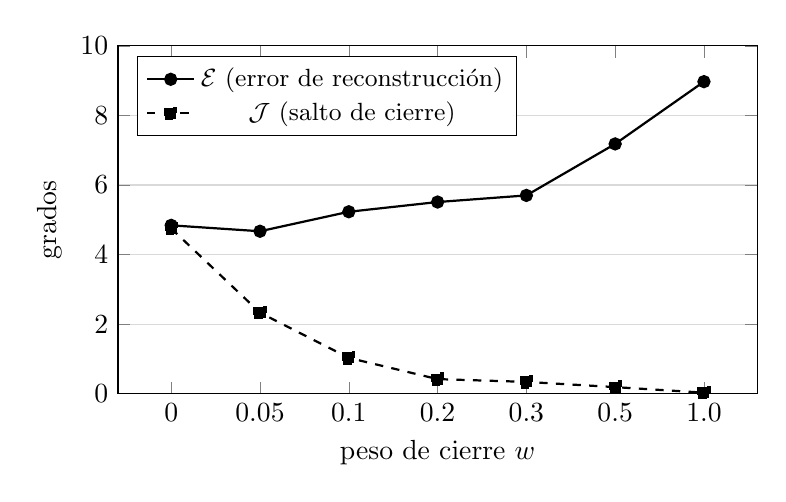
\begin{tikzpicture}
\begin{axis}[width=0.8\textwidth,height=6cm,xlabel={peso de cierre $w$},ylabel={grados},
 symbolic x coords={0,0.05,0.1,0.2,0.3,0.5,1.0},xtick=data,ymin=0,ymax=10,legend pos=north west,
 ymajorgrids,grid style={gray!30},legend style={font=\small}]
\addplot[color=black,mark=*,thick] coordinates {(0,4.84)(0.05,4.67)(0.1,5.23)(0.2,5.51)(0.3,5.70)(0.5,7.18)(1.0,8.97)};
\addlegendentry{$\mathcal E$ (error de reconstrucción)}
\addplot[color=black,mark=square*,thick,dashed] coordinates {(0,4.75)(0.05,2.33)(0.1,1.03)(0.2,0.42)(0.3,0.34)(0.5,0.19)(1.0,0.03)};
\addlegendentry{$\mathcal J$ (salto de cierre)}
\end{axis}
\end{tikzpicture}
\caption{Resultado R4: compromiso entre fidelidad y cierre al variar el peso $w$ (modelo A con código en cada paso, una semilla).}
\label{fig:w}
\end{figure}

Con las dos modificaciones y $d=16$, $w=0.05$, el error es $4.20\pm0.03$\gr{} y el salto $1.33\pm0.15$\gr{}, y la combinación gana en las cinco semillas en ambas métricas frente al original. Al pasar a $d=32$ y reajustar $w=0.1$, el error baja a $4.11\pm0.05$\gr{} ($p=0.018$ frente a $d=16$) y el salto a $0.87\pm0.11$\gr{} ($p=0.004$): el mejor $w$ depende del tamaño del código.

\subsection{R5. Ensambles}
\label{sec:r5}

\textit{Métodos: sección~\ref{sec:modelos}. Hipótesis: H4.} La tabla~\ref{tab:ens} compara cada modelo con el ensamble de sus cinco semillas. En las ocho comparaciones (A y B, originales y mejorados, error y salto), el ensamble tiene un valor menor que el promedio de sus miembros. En A mejorado el error pasa de $4.11$\gr{} a $3.91$\gr{} y el salto de $0.87$\gr{} a $0.55$\gr{}; en B mejorado, de $4.83$\gr{} a $4.74$\gr{} y de $0.57$\gr{} a $0.36$\gr{}, con una ganancia de corrección de $0.349$. Cada ensamble es único y su incertidumbre no se midió, por lo que H4 se evalúa de forma descriptiva y no se contrastó con una prueba.

\begin{table}[h]
\centering\small
\setlength{\tabcolsep}{3pt}
\begin{tabular}{llcccc}
\toprule
 & & $\mathcal E$ (\gr) & $\mathcal J$ (\gr) & $\gamma$ & Tipicidad \\
\midrule
\multirow{2}{*}{A original} & 1 modelo & $4.99\pm0.23$ & $5.07\pm0.55$ & $0.208\pm0.018$ & $0.345\pm0.008$ \\
 & Ensamble & 4.81 & 4.50 & 0.249 & 0.362 \\
\multirow{2}{*}{A mejorado} & 1 modelo & $4.11\pm0.05$ & $0.87\pm0.11$ & $0.189\pm0.012$ & $0.326\pm0.007$ \\
 & Ensamble & 3.91 & 0.55 & 0.229 & 0.358 \\
\multirow{2}{*}{B original} & 1 modelo & $5.25\pm0.10$ & $3.04\pm0.31$ & $0.296\pm0.014$ & $0.383\pm0.004$ \\
 & Ensamble & 5.19 & 2.72 & 0.305 & 0.392 \\
\multirow{2}{*}{B mejorado} & 1 modelo & $4.83\pm0.07$ & $0.57\pm0.05$ & $0.337\pm0.007$ & $0.414\pm0.008$ \\
 & Ensamble & 4.74 & 0.36 & 0.349 & 0.423 \\
\bottomrule
\end{tabular}
\caption{Resultado R5: modelo individual (media $\pm$ desviación estándar de cinco semillas) y ensamble de esas cinco semillas.}
\label{tab:ens}
\end{table}

\subsection{R6. Regularizaciones de diferencias consecutivas}
\label{sec:r6}

\textit{Métodos: sección~\ref{sec:fm_met}. Hipótesis: ninguna (exploración de la sugerencia de penalizar la diferencia entre $t$ y $t-1$).} Penalizar la suavidad o la aceleración de forma convencional, sin la costura, no cambió el error con pesos pequeños y lo empeoró con pesos grandes (4.219\gr{}, 4.215\gr{} y 4.451\gr{} con pesos 0, 0.2 y 3.0). Las lecturas circulares se validaron con cinco semillas en el modelo A con $d=16$ (tabla~\ref{tab:lecturas}). Frente a la referencia con el mismo $w=0.1$, igualar incrementos reduce el error ($p=0.008$), la pendiente en la costura ($-39\%$), el error en los incrementos ($-4\%$) y la rugosidad ($-7\%$), todos con $p<0.01$, a cambio de un salto mayor (de $0.83$\gr{} a $0.99$\gr{}, $p=0.005$). La mejora de error ($0.03$\gr) es detectable pero sin importancia práctica. En el modelo B el patrón se repite: la pendiente en la costura baja de $1.03\pm0.17$ a $0.58\pm0.06$ con incrementos ($p=0.002$) sin cambio en el error ni en la corrección. El núcleo periódico y el peso por fase no ayudan.

\begin{table}[h]
\centering\footnotesize
\setlength{\tabcolsep}{3pt}
\begin{tabular}{lccccc}
\toprule
 & $\mathcal E$ & $\mathcal J$ & Pend. costura & Err. increm. & Rugosidad \\
\midrule
Referencia, $w=0.05$ & $4.196\pm0.025$ & $1.33\pm0.15$ & $1.15\pm0.19$ & $0.578\pm0.007$ & $0.118\pm0.003$ \\
Referencia, $w=0.1$ & $4.244\pm0.031$ & $0.83\pm0.07$ & $1.15\pm0.16$ & $0.581\pm0.008$ & $0.118\pm0.004$ \\
Incrementos, $w=0.1$ & $4.212\pm0.032$ & $0.99\pm0.12$ & $0.70\pm0.09$ & $0.557\pm0.005$ & $0.110\pm0.002$ \\
Incrementos y curvatura, $w=0.1$ & $4.214\pm0.026$ & $0.95\pm0.10$ & $0.58\pm0.07$ & $0.553\pm0.003$ & $0.104\pm0.002$ \\
Incrementos y pendiente, $w=0.1$ & $4.244\pm0.056$ & $0.96\pm0.06$ & $0.19\pm0.02$ & $0.553\pm0.006$ & $0.106\pm0.001$ \\
Curvatura (peso 3), $w=0.05$ & $4.248\pm0.031$ & $0.96\pm0.09$ & $0.52\pm0.04$ & $0.567\pm0.007$ & $0.094\pm0.002$ \\
\midrule
Ciclos reales (referencia) & -- & 6.0 & 0.81 & -- & 0.226 \\
\bottomrule
\end{tabular}
\caption{Resultado R6: lecturas circulares de la sugerencia, modelo A con $d=16$, cinco semillas (grados). Menor es mejor en todas las columnas.}
\label{tab:lecturas}
\end{table}

\subsection{R7. Componentes que no mejoraron el modelo}
\label{sec:r7}

\textit{Métodos: sección~\ref{sec:fm_met}. Hipótesis: ninguna (delimitación del cuello de botella).} Casi todos los componentes aprendibles añadidos no mejoraron el modelo (tabla~\ref{tab:neg}).

\begin{table}[h]
\centering\footnotesize
\begin{tabularx}{\textwidth}{@{}>{\raggedright\arraybackslash}p{3.6cm}>{\raggedright\arraybackslash}X@{}}
\toprule
Componente & Resultado \\
\midrule
Decodificador bidireccional & Error 4.244\gr{} y salto 3.920\gr{} (sin cierre) y 4.273\gr{} y 1.072\gr{} (con cierre), frente a 4.219\gr{} y 3.912\gr{} y 4.182\gr{} y 1.140\gr{} con el unidireccional. \\
Atención en el codificador & Error de unos 8.5\gr{}; pesos de atención casi uniformes (cerca de $1/101$). Con temperatura muy baja, 5.6\gr. \\
Velocidad angular como entrada (B) & Error $4.728\to4.822$\gr{} (peor). \\
Asimetría izquierda-derecha (B) & Error $4.728\to4.771$\gr{}; corrección $0.349\to0.333$. \\
Consistencia del código (B) & Peso 0.05: error 4.833 frente a 4.835\gr{}, corrección 0.320 frente a 0.322 ($p=0.85$ y $0.40$); con peso 0.5, error 4.935\gr. \\
Intensidad del daño (B) & Con 0.5, 1.0 y 1.5: error 4.45, 4.73 y 5.12\gr{}; corrección 0.320, 0.349 y 0.329. \\
Currículo de daño (B) & Error $4.83\to4.79$\gr{}, corrección $0.320\to0.324$ ($p=0.26$ y $0.51$). \\
\bottomrule
\end{tabularx}
\caption{Resultado R7: componentes adicionales sin mejora apreciable.}
\label{tab:neg}
\end{table}

\subsection{R8. Codificador fundacional congelado}
\label{sec:r8}

\textit{Métodos: sección~\ref{sec:fm_met}. Hipótesis: H5.} La exploración en validación dio errores de $7.43$\gr{} a $8.28$\gr{} entre las ocho configuraciones (apéndice~\ref{app:timesfm}) y se eligieron el décimo bloque, la agrupación de promedio y último parche y un decaimiento de pesos de $10^{-3}$. La verificación de la carga de pesos, que consiste en pronosticar 32 puntos de una onda seno, dio un error medio absoluto de $0.036$ con los pesos preentrenados y de $1.877$ con pesos aleatorios. La tabla~\ref{tab:fm} y la figura~\ref{fig:fm} presentan el resultado en prueba.

\begin{table}[h]
\centering\footnotesize
\setlength{\tabcolsep}{2.5pt}
\begin{tabular}{llccccc}
\toprule
 & & $\mathcal E$ (\gr) & $\mathcal J$ (\gr) & $\gamma$ & Tipicidad & Interv. (\gr) \\
\midrule
\multicolumn{7}{l}{\textit{Tipo A (ciclos limpios)}}\\
TimesFM preentrenado & & $7.19\pm0.22$ & $2.55\pm0.15$ & $-0.149\pm0.019$ & $0.101\pm0.022$ & $9.22\pm0.13$ \\
 & ensamble & 6.76 & 1.41 & $-0.117$ & 0.147 & 8.87 \\
TimesFM pesos aleatorios & & $7.23\pm0.48$ & $2.74\pm0.17$ & $-0.017\pm0.042$ & $0.087\pm0.042$ & $9.34\pm0.23$ \\
 & ensamble & 6.66 & 1.59 & 0.045 & 0.153 & 8.82 \\
Serie cruda (lineal) & & $3.69\pm0.11$ & $1.40\pm0.05$ & $0.011\pm0.021$ & $0.181\pm0.013$ & $5.45\pm0.09$ \\
 & ensamble & 3.26 & 0.81 & 0.083 & 0.236 & 4.89 \\
GRU mejorado (referencia) & & $4.11\pm0.05$ & $0.87\pm0.11$ & $0.189\pm0.012$ & $0.326\pm0.007$ & $6.14\pm0.10$ \\
 & ensamble & 3.91 & 0.55 & 0.229 & 0.358 & 5.89 \\
\midrule
\multicolumn{7}{l}{\textit{Tipo B (con eliminación de ruido)}}\\
TimesFM preentrenado & & $10.12\pm0.18$ & $6.80\pm2.05$ & $-0.117\pm0.110$ & $-0.049\pm0.028$ & $11.47\pm0.04$ \\
 & ensamble & 9.76 & 3.32 & $-0.050$ & $-0.015$ & 11.16 \\
Serie cruda (lineal) & & $4.46\pm0.06$ & $1.28\pm0.13$ & $0.380\pm0.010$ & $0.390\pm0.008$ & $6.55\pm0.08$ \\
 & ensamble & 4.33 & 0.91 & 0.405 & 0.413 & 6.40 \\
GRU mejorado (referencia) & & $4.83\pm0.07$ & $0.57\pm0.05$ & $0.337\pm0.007$ & $0.414\pm0.008$ & $7.09\pm0.10$ \\
 & ensamble & 4.74 & 0.36 & 0.349 & 0.423 & 7.01 \\
\bottomrule
\end{tabular}
\caption{Resultados R8 y R9: codificador fundacional congelado y controles, con el mismo decodificador y protocolo. Media $\pm$ desviación estándar de cinco semillas y, en la fila siguiente, ensamble de las cinco. El control de pesos aleatorios es el corregido (escalas de las normas fijadas en uno).}
\label{tab:fm}
\end{table}

\begin{figure}[h]
\centering
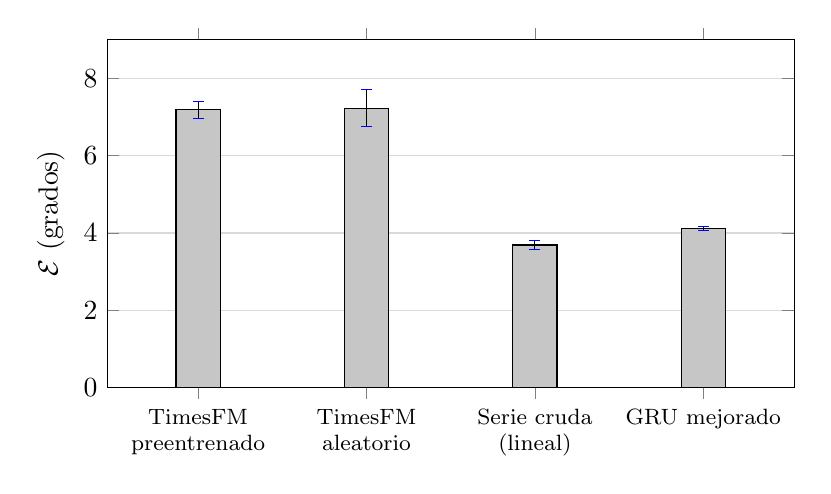
\begin{tikzpicture}
\begin{axis}[ybar,bar width=16pt,width=0.85\textwidth,height=6cm,ylabel={$\mathcal E$ (grados)},
 symbolic x coords={pre,ale,cru,gru},xtick=data,
 xticklabels={TimesFM preentrenado,TimesFM aleatorio,Serie cruda (lineal),GRU mejorado},
 x tick label style={font=\footnotesize,text width=2.3cm,align=center},enlarge x limits=0.18,ymin=0,ymax=9,
 ymajorgrids,grid style={gray!30},error bars/y dir=both,error bars/y explicit]
\addplot+[fill=gray!45,draw=black] coordinates {(pre,7.19) +- (0,0.22) (ale,7.23) +- (0,0.48) (cru,3.69) +- (0,0.11) (gru,4.11) +- (0,0.05)};
\end{axis}
\end{tikzpicture}
\caption{Resultado R8: error de reconstrucción $\mathcal E$ en el tipo A para el codificador fundacional preentrenado, el mismo con pesos aleatorios, la proyección lineal de la serie cruda y el GRU mejorado. Barras de error: una desviación estándar entre cinco semillas.}
\label{fig:fm}
\end{figure}

La tabla~\ref{tab:fmd} presenta las diferencias pareadas. El preentrenamiento no mejora la fidelidad: el error con pesos preentrenados es igual al de pesos aleatorios (diferencia $-0.05\pm0.58$\gr, $p=0.83$). El salto no difiere de forma significativa ($p=0.19$) y la ganancia de corrección es peor con pesos preentrenados ($p=0.004$). Frente al GRU mejorado, el codificador fundacional es peor en fidelidad, cierre, corrección y tipicidad en ambos tipos ($p\le0.003$). En el tipo B el entrenamiento se detuvo pronto (entre 20 y 42 épocas) y la corrección fue negativa. H5 no se cumple en este diseño. Una primera versión del control de pesos aleatorios dio un error de $7.14$\gr{}, y la versión corregida $7.23$\gr; la conclusión no cambió.

\begin{table}[h]
\centering\small
\setlength{\tabcolsep}{3pt}
\begin{tabular}{llcccc}
\toprule
Tipo & Comparación (primero $-$ segundo) & $\mathcal E$ (\gr) & $\mathcal J$ (\gr) & $\gamma$ & Tipicidad \\
\midrule
A & Preentrenado $-$ aleatorio & $-0.05\pm0.58$ & $-0.19\pm0.33$ & $-0.132\pm0.060$ & $+0.013\pm0.057$ \\
 & Valor $p$ & 0.83 & 0.19 & 0.004 & 0.55 \\
A & Preentrenado $-$ GRU mejorado & $+3.07\pm0.23$ & $+1.68\pm0.28$ & $-0.338\pm0.029$ & $-0.226\pm0.025$ \\
 & Valor $p$ & $<0.001$ & $<0.001$ & $<0.001$ & $<0.001$ \\
B & Preentrenado $-$ GRU mejorado & $+5.29\pm0.28$ & $+6.23\pm2.55$ & $-0.454\pm0.144$ & $-0.463\pm0.035$ \\
 & Valor $p$ & $<0.001$ & 0.003 & $<0.001$ & $<0.001$ \\
\bottomrule
\end{tabular}
\caption{Resultado R8: diferencias pareadas por semilla con la semiamplitud del intervalo de confianza de 95\% (cinco semillas, $\alpha=0.05$, sin corrección por multiplicidad). Para $\mathcal E$ y $\mathcal J$, un valor positivo indica que el primer modelo es peor; para $\gamma$ y la tipicidad, un valor negativo indica que el primer modelo es peor.}
\label{tab:fmd}
\end{table}

\subsection{R9. Control: un codificador lineal de la serie cruda}
\label{sec:r9}

\textit{Métodos: sección~\ref{sec:fm_met}. Hipótesis: H5 (control no planeado como hipótesis).} La proyección lineal de la serie cruda, con el mismo decodificador, tiene un error menor que el del GRU mejorado en el tipo A ($3.69$\gr{} frente a $4.11$\gr, diferencia $-0.43\pm0.17$\gr, $p=0.002$) y en el tipo B ($4.46$\gr{} frente a $4.83$\gr, diferencia $-0.37\pm0.08$\gr, $p<0.001$), y una mayor ganancia de corrección en el tipo B ($0.380$ frente a $0.337$, $p<0.001$). En cambio es peor en salto de cierre (diferencias de $+0.53\pm0.18$\gr{} en A y $+0.72\pm0.13$\gr{} en B), en la pendiente en la costura y, en el tipo A, en corrección y tipicidad ($p<0.001$). El resultado surgió de un control y no de una hipótesis previa.

\subsection{R10. Resumen del contraste de hipótesis}
\label{sec:r10}

\begin{table}[h]
\centering\small
\begin{tabularx}{\textwidth}{@{}l>{\raggedright\arraybackslash}X>{\raggedright\arraybackslash}p{4.6cm}@{}}
\toprule
Hipótesis & Evidencia & Decisión \\
\midrule
H1 & Una semilla de forma aislada (R4); cinco semillas en la combinación con la pérdida de cierre (R2, R3). & Apoyada en la combinación; no contrastada de forma aislada. \\
H2 & Cinco semillas en la combinación (R2): $\mathcal J$ baja con $p<0.001$ y $\mathcal E$ no empeora; barrido de $w$ con una semilla (R4). & Apoyada; el $w$ adecuado depende de $d$. \\
H3 & Cinco semillas, prueba t pareada (R3): $\mathcal J$ ($p<0.001$) y $\gamma$ ($p=0.002$). & Apoyada. \\
H4 & Ocho comparaciones descriptivas, un ensamble por configuración (R5). & Cumplida en las ocho; sin prueba ni incertidumbre. \\
H5 & Cinco semillas, con dos controles (R8, R9). & No apoyada: $\mathcal E$ y $\gamma$ peores ($p\le0.003$). \\
\bottomrule
\end{tabularx}
\caption{Resultado R10: estado de las hipótesis.}
\label{tab:hipres}
\end{table}

%====================================================================
\section{Discusión}
\label{sec:discusion}

Las interpretaciones de esta sección se apoyan en principios o modelos enunciados explícitamente y se indica cuáles se contrastaron con los datos y cuáles son solo coherentes con ellos.

\subsection{Cierre del ciclo como compromiso entre fidelidad y periodicidad}

Minimizar $\mathcal E+w\,\mathcal J$ para $w\ge0$ es una escalarización del problema de optimización con dos objetivos, y recorre la parte soportada de la frontera de Pareto entre fidelidad y cierre \cite{boyd2004}. La figura~\ref{fig:w} es la versión empírica de esa frontera. Entre $w=0.1$ y $w=0.5$, el error sube $1.95$\gr{} para reducir el salto en $0.84$\gr{}, un costo de unos $2.3$\gr{} de error por grado de salto, mientras que entre $w=0$ y $w=0.1$ el costo es de $0.10$\gr{} por grado (cifras de una sola semilla, por lo que son orientativas). Una frontera con costo marginal creciente es lo esperado cuando los extremos se pueden cerrar con poco costo de fidelidad al principio y con un costo creciente al exigir un cierre casi exacto.

Hay además un argumento de escala. Si el cierre se lograra moviendo solo los dos puntos extremos de cada canal, el cambio en el error absoluto medio sería del orden de $(|\delta_1|+|\delta_{101}|)/101$, con $\delta$ el desplazamiento de cada extremo; con desplazamientos del orden de la reducción del salto ($4.2$\gr) el cambio sería de unos $0.08$\gr{}, mucho menor que la reducción de $0.88$\gr{} observada en el modelo A. Esto es coherente con que la mejora de fidelidad provenga sobre todo de la modificación 1 y no del cierre, lo que concuerda con el resultado exploratorio de una semilla (R4), aunque la descomposición con cinco semillas no se hizo.

También conviene tener presente que los ciclos reales de control no cierran (salto medio de unos $6$\gr). Un modelo con $\mathcal J\approx0.9$\gr{} produce ciclos más periódicos que los datos que reconstruye. La pérdida de cierre impone, por tanto, una propiedad deseada (periodicidad) y no fidelidad a la medición, que incluye el ruido de la estimación de ángulos a partir de video \cite{kidzinski2020}.

\subsection{Código en cada paso del decodificador}

En el decodificador original la sensibilidad del estado al código es $\partial h_t/\partial z=(\prod_{k=1}^{t}J_k)W_0$ con $J_k=\partial h_k/\partial h_{k-1}$; si $\|J_k\|\le\rho<1$ la influencia decae al menos como $\rho^t$ (con $\rho=0.95$ y $t=100$, $0.006$). Al entregar $z$ en cada paso aparece un término de longitud uno, que no atraviesa productos de jacobianos, como en el decodificador de \cite{cho2014}. La dificultad de las redes recurrentes para propagar información a lo largo de muchos pasos está documentada \cite{pascanu2013}. Este mecanismo es coherente con dos hechos observados: la reducción del error de reconstrucción y la reducción de la dispersión entre semillas del error (de $0.23$\gr{} a $0.05$\gr{} en A), que es la esperada si la optimización se vuelve menos dependiente de la inicialización. Sin embargo, no se midió la norma de los jacobianos, de modo que el mecanismo no se verificó; otras explicaciones, como el simple aumento del tamaño del código de 16 a 32 en A, no se separaron por completo (el paso de $d=16$ a $d=32$ aporta $0.08$\gr).

\subsection{Corrección, tipicidad e intervención}

El modelo B mejora en corrección ($0.296\to0.337$) y el A no ($0.208\to0.189$, $p=0.077$). Es lo esperado según el principio del autoencoder con eliminación de ruido \cite{vincent2008}: la capacidad de proyectar entradas dañadas hacia la variedad de ciclos típicos se aprende al entrenar con entradas dañadas, y el modelo A nunca las vio, de modo que su ganancia de corrección proviene únicamente del cuello de botella. La caída de la ganancia de tipicidad del modelo A ($0.345\to0.326$, $p=0.034$) se relaciona con la caída de la intervención ($7.78\to6.14$\gr): una función identidad da intervención y ganancia de tipicidad nulas, y un modelo que reproduce con mayor fidelidad también reproduce con mayor fidelidad los rasgos atípicos de los ciclos de casos, que no se acercan tanto a los controles. Esta relación es coherente con los datos y no se probó como causal.

\subsection{Ensambles}

Para un ensamble de $M$ modelos, la desigualdad de Jensen garantiza que, para cualquier pérdida convexa en la predicción como el error absoluto, $\|\bar f-G\|_1\le\frac1M\sum_m\|f_m-G\|_1$; lo mismo ocurre con el salto de cierre, que es una combinación de valores absolutos de funciones lineales de la predicción. Las ocho desigualdades de R5 se cumplen, como debían, y por ello constituyen una comprobación de la implementación y no una confirmación empírica de H4. Para el error cuadrático, la identidad de ambigüedad $\frac1M\sum_m\|f_m-G\|^2=\|\bar f-G\|^2+\frac1M\sum_m\|f_m-\bar f\|^2$ \cite{krogh1995} muestra que la ganancia del ensamble es exactamente la diversidad entre sus miembros; con $\Mae$ solo se tiene una cota. La magnitud observada es pequeña en B ($0.09$\gr) y mayor en A ($0.20$\gr), lo que sugiere menor diversidad entre los miembros de B, aunque con un solo ensamble por configuración no puede afirmarse.

\subsection{Por qué un codificador lineal es competitivo}

Para una matriz de datos centrada $X\in\R^{n\times p}$ con $n=240$ y $p=606$, el teorema de Eckart y Young \cite{eckart1936} establece que la mejor aproximación de rango $k$ en norma de Frobenius es la descomposición en valores singulares truncada, es decir, PCA \cite{jolliffe2016}, y que el rango de $X$ no pasa de $239$. Con pocas muestras, el sesgo de un modelo lineal es bajo si los ciclos están cerca de un subespacio de baja dimensión y su varianza es menor que la de un modelo no lineal; en la descomposición del error de predicción en ruido, sesgo cuadrado y varianza \cite{hastie2009}, la varianza domina cuando $n$ es pequeño. Esto es coherente con tres observaciones: el buen desempeño de PCA en la comparación inicial (2.78\gr), el menor error de la proyección lineal con el decodificador recurrente (3.69\gr{} frente a 4.11\gr) y la ausencia de mejora de la mayoría de los componentes añadidos (R7). Los hiperparámetros del GRU se ajustaron en el conjunto de prueba de control y los del control lineal no, por lo que la comparación favorece al GRU, que aun así pierde en error. No se midieron curvas de aprendizaje, por lo que la interpretación de que el tamaño de los datos es el límite es coherente con las observaciones, pero no es una conclusión.

\subsection{Por qué el modelo fundacional congelado no ayudó}

El resultado decisivo es que el error con pesos preentrenados (7.19\gr) no difiere del de pesos aleatorios (7.23\gr; $p=0.83$). Con una proyección lineal sobre las características agrupadas de una red con pesos fijos, el modelo es un modelo de características aleatorias \cite{rahimi2007}, que aproxima un método de núcleo; si el preentrenamiento no cambia el resultado, las representaciones preentrenadas no contienen, bajo este protocolo, más información útil para reconstruir el ciclo que una expansión aleatoria. Se identifican cuatro causas posibles, todas hipótesis no medidas. Primera, TimesFM normaliza internamente cada serie por instancia, lo que elimina su nivel y su escala \cite{kim2022revin}; se añadieron la media y la desviación estándar para compensarlo, pero la forma fina del ciclo puede perderse al promediar los parches. Segunda, el preentrenamiento optimiza el pronóstico del siguiente parche \cite{das2024timesfm}, y las representaciones intermedias codifican información predictiva y no necesariamente la forma exacta de la onda. Tercera, el remuestreo de 101 a 128 puntos da solo cuatro parches, un contexto mucho menor que aquel para el que se diseñó el modelo (hasta 16\,000 puntos \cite{timesfm25}). Cuarta, la cabeza lineal tiene $15\,372\times32$ parámetros para $240$ ciclos, y aunque el decaimiento de pesos regulariza, el problema está muy sobreparametrizado. La verificación con la onda seno (error de $0.036$ con pesos preentrenados y $1.877$ con aleatorios) indica que el modelo funciona para pronóstico, de modo que el resultado negativo no se atribuye a un fallo de carga de pesos. Por último, el error de un diseño de uso no debe extenderse a otros: no se probaron los parches sin promediar, otros modelos como MOMENT o Chronos \cite{goswami2024moment,ansari2024chronos} ni el ajuste fino.

\subsection{Relación con la literatura}

La modificación 1 reproduce en el decodificador la forma original del codificador-decodificador recurrente, donde el contexto condiciona cada paso \cite{cho2014}; hasta donde alcanza la revisión del Informe 1, su evaluación en ciclos de marcha, con partición por sujeto y varias semillas, es lo que aporta este trabajo. La periodicidad se impone aquí con una pérdida de cierre, y no en la estructura del código latente como en el autoencoder periódico \cite{starke2022}; no se compararon ambos enfoques. Frente a los autoencoders aplicados a marcha en parálisis cerebral, que se evalúan como índices resumen o como clasificadores de fase \cite{wang2024,pang2025}, este trabajo evalúa la reconstrucción de ciclos completos. Por último, el tamaño de la muestra y la dependencia de una sola partición son limitaciones señaladas en las revisiones del área \cite{samadi2024}, y este estudio las comparte.

\subsection{Aportes}

\begin{enumerate}
\item Un diagnóstico de dos limitaciones del autoencoder recurrente (dilución del código a lo largo del decodificador y ausencia de periodicidad) con un argumento formal y su corrección con dos modificaciones, que reducen el salto de cierre en $82.9\%$ (A) y $81.4\%$ (B) y el error en $17.6\%$ (A) y $8.0\%$ (B), con cinco semillas y prueba pareada.
\item Un protocolo reproducible, con partición por sujeto, cinco semillas, diferencias pareadas con intervalo de confianza y métricas de forma, publicado con el código y los resultados.
\item Un resultado negativo documentado: el codificador fundacional congelado no mejora el modelo y es indistinguible de pesos aleatorios, con el hallazgo adicional de que una proyección lineal de la serie cruda supera al codificador recurrente en error.
\item Una verificación de implementación del control con pesos aleatorios, cuyo defecto inicial (escalas de normalización en cero) se detectó, se corrigió y se informó.
\end{enumerate}

\subsection{Limitaciones}

\begin{enumerate}
\item \textit{Selección de hiperparámetros sobre el conjunto de prueba de control.} El peso $w$ y el tamaño del código se eligieron observando el conjunto en el que se reportan los resultados, por lo que las cifras del GRU son algo optimistas. La configuración del modelo fundacional se eligió solo con validación.
\item \textit{Tamaño y filtro de los datos.} El entrenamiento usa 240 ciclos de 28 sujetos; el control de calidad descartó cerca de 17\% de los 551 intervalos y no hay un conjunto externo independiente. Los ciclos de una persona no son independientes entre sí.
\item \textit{Alcance de la prueba t.} Con cinco semillas se mide la variabilidad por inicialización y por orden de lotes, no por muestreo de sujetos. Se probaron muchas variantes sin corrección por comparaciones múltiples, y los valores $p$ deben leerse con cautela; los intervalos de confianza con $t_4$ son anchos.
\item \textit{Efectos aislados.} Las modificaciones 1 y 2 se contrastaron por separado solo con una semilla.
\item \textit{Ensambles.} Cada ensamble proviene de un único conjunto de cinco modelos y no se midió su variabilidad.
\item \textit{Evaluación de corrección.} La ganancia $\gamma$ usa una sola realización del daño; con realizaciones distintas por semilla, la corrección del modelo B mejorado fue $0.32\pm0.02$ frente a $0.337\pm0.007$ con la realización fija, una variabilidad de orden $0.02$.
\item \textit{Modelos de referencia.} PCA, el proceso gaussiano y los autoencoders convolucionales proceden de una sola corrida de la comparación inicial y no se ajustaron con el mismo esfuerzo; no se compararon con cinco semillas.
\item \textit{Datos reconstruidos y daño sintético.} Los datos derivados se reconstruyeron a partir de los archivos entregados, y el daño sintético no representa necesariamente una marcha patológica real; la tipicidad mide cercanía a controles, no corrección clínica.
\item \textit{Modelo fundacional.} Se evaluó un solo modelo y un solo diseño de uso, con ocho configuraciones y una semilla de exploración; los experimentos con TimesFM se ejecutaron en un entorno de GPU distinto del de los GRU.
\item \textit{Procedencia y ética.} La etiqueta control o caso proviene del reporte de migración del proyecto; el protocolo ético y de consentimiento debe confirmarse con el tutor científico antes de cualquier difusión.
\end{enumerate}

%====================================================================
\section{Conclusiones y trabajo futuro}
\label{sec:conclusiones}

Entregar el código latente en cada paso del decodificador y añadir un término de cierre a la pérdida redujeron, en cinco semillas y con ciclos de control no vistos, el salto de cierre en más de $80\%$ y el error de reconstrucción en $17.6\%$ (modelo A) y $8.0\%$ (modelo B), con una dispersión entre semillas menor, y aumentaron la ganancia de corrección de la variante con eliminación de ruido de $0.296$ a $0.337$. La mejora del modelo A es de fidelidad y de cierre, no de corrección ni de tipicidad. Los ensambles reducen el error y el salto, como corresponde a la convexidad de ambas métricas, pero su incertidumbre no se midió. La mayoría de los componentes añadidos no aportó, y un codificador fundacional de series de tiempo congelado (TimesFM 2.5) no mejoró los resultados: su error fue igual al de pesos aleatorios y mayor que el del GRU. Una proyección lineal de la serie cruda tuvo un menor error de reconstrucción que el codificador recurrente, por lo que no hay evidencia de que este sea necesario para reconstruir ciclos. Estas conclusiones se limitan a un conjunto de 240 ciclos de entrenamiento, a un solo diseño de uso del modelo fundacional y a hiperparámetros ajustados sobre el conjunto de prueba de control.

Las dificultades principales fueron la reconstrucción de los datos derivados, que dio cifras ligeramente distintas de las iniciales; la imposibilidad de ejecutar el modelo fundacional preentrenado en el entorno de desarrollo, que obligó a usar un entorno de GPU externo; y un defecto en la primera versión del control con pesos aleatorios, que se corrigió y se repitió.

Como trabajo futuro se proponen: (i) elegir hiperparámetros por validación cruzada por sujeto y reportar la prueba una sola vez; (ii) medir el codificador lineal con ajuste propio, con las mejoras de cierre, frente a PCA y al autoencoder convolucional, con el mismo protocolo de cinco semillas; (iii) separar con cinco semillas el efecto del código en cada paso del de la pérdida de cierre y del tamaño del código; (iv) trazar curvas de aprendizaje para contrastar la interpretación del límite impuesto por los datos; (v) probar variantes del modelo fundacional (parches sin promediar, otros modelos, ajuste fino) y la comparación con la periodicidad en el espacio latente \cite{starke2022}; (vi) repetir los ensambles para medir su incertidumbre; y (vii) definir con criterio clínico qué error de reconstrucción o de corrección es suficiente para la aplicación.

\section*{Disponibilidad de código y resultados}

El código, los cuadernos ejecutados y los resultados por semilla se encuentran en el repositorio \texttt{github.com/JDavidCE2022/gait-cycle-manifold}, que no incluye los datos (se describen en \texttt{data/README.md}). Las tablas de los resultados R2, R3 y R8 provienen de los archivos de la carpeta \texttt{results/}.

%====================================================================
\begin{thebibliography}{99}
\small
\bibitem{neurostride2026} Proyecto NeuroStrideAI, ``Formulación matemática de los modelos: manifold de marcha control y modelo normativo por fase,'' registro de trabajo del proyecto, 23 de septiembre de 2026.
\bibitem{hinton2006} G. E. Hinton y R. R. Salakhutdinov, ``Reducing the dimensionality of data with neural networks,'' \emph{Science}, vol. 313, no. 5786, pp. 504--507, 2006.
\bibitem{vincent2008} P. Vincent, H. Larochelle, Y. Bengio y P.-A. Manzagol, ``Extracting and composing robust features with denoising autoencoders,'' en \emph{Proc. ICML}, 2008, pp. 1096--1103.
\bibitem{cho2014} K. Cho et al., ``Learning phrase representations using RNN encoder--decoder for statistical machine translation,'' en \emph{Proc. EMNLP}, 2014, pp. 1724--1734.
\bibitem{schuster1997} M. Schuster y K. K. Paliwal, ``Bidirectional recurrent neural networks,'' \emph{IEEE Transactions on Signal Processing}, vol. 45, no. 11, pp. 2673--2681, 1997.
\bibitem{pascanu2013} R. Pascanu, T. Mikolov y Y. Bengio, ``On the difficulty of training recurrent neural networks,'' en \emph{Proc. ICML}, PMLR vol. 28, pp. 1310--1318, 2013.
\bibitem{fang2023alphapose} H.-S. Fang, J. Li, H. Tang, C. Xu, H. Zhu, Y. Xiu, Y.-L. Li y C. Lu, ``AlphaPose: whole-body regional multi-person pose estimation and tracking in real-time,'' \emph{IEEE Transactions on Pattern Analysis and Machine Intelligence}, 2023 (arXiv:2211.03375).
\bibitem{fritsch1980} F. N. Fritsch y R. E. Carlson, ``Monotone piecewise cubic interpolation,'' \emph{SIAM Journal on Numerical Analysis}, vol. 17, no. 2, pp. 238--246, 1980.
\bibitem{saeb2017} S. Saeb, L. Lonini, A. Jayaraman, D. C. Mohr y K. P. Kording, ``The need to approximate the use-case in clinical machine learning,'' \emph{GigaScience}, vol. 6, no. 5, gix019, 2017.
\bibitem{dietterich2000} T. G. Dietterich, ``Ensemble methods in machine learning,'' en \emph{Multiple Classifier Systems}, LNCS 1857, Springer, 2000, pp. 1--15.
\bibitem{bahdanau2015} D. Bahdanau, K. Cho y Y. Bengio, ``Neural machine translation by jointly learning to align and translate,'' en \emph{Proc. ICLR}, 2015.
\bibitem{das2024timesfm} A. Das, W. Kong, R. Sen y Y. Zhou, ``A decoder-only foundation model for time-series forecasting,'' en \emph{Proc. 41st International Conference on Machine Learning}, PMLR vol. 235, pp. 10148--10167, 2024.
\bibitem{timesfm25} Google Research, ``TimesFM 2.5 (200 millones de parámetros),'' repositorio y ficha del modelo, github.com/google-research/timesfm, actualización del 15 de septiembre de 2025.
\bibitem{goswami2024moment} M. Goswami, K. Szafer, A. Choudhry, Y. Cai, S. Li y A. Dubrawski, ``MOMENT: a family of open time-series foundation models,'' en \emph{Proc. 41st International Conference on Machine Learning}, PMLR vol. 235, pp. 16115--16152, 2024.
\bibitem{ansari2024chronos} A. F. Ansari et al., ``Chronos: learning the language of time series,'' \emph{Transactions on Machine Learning Research}, 2024 (arXiv:2403.07815).
\bibitem{kim2022revin} T. Kim, J. Kim, Y. Tae, C. Park, J.-H. Choi y J. Choo, ``Reversible instance normalization for accurate time-series forecasting against distribution shift,'' en \emph{Proc. ICLR}, 2022.
\bibitem{paszke2019} A. Paszke et al., ``PyTorch: an imperative style, high-performance deep learning library,'' en \emph{Advances in Neural Information Processing Systems 32}, 2019.
\bibitem{kingma2015} D. P. Kingma y J. Ba, ``Adam: a method for stochastic optimization,'' en \emph{Proc. ICLR}, 2015.
\bibitem{prechelt1998} L. Prechelt, ``Early stopping -- but when?,'' en \emph{Neural Networks: Tricks of the Trade}, LNCS 1524, Springer, 1998, pp. 55--69.
\bibitem{jolliffe2016} I. T. Jolliffe y J. Cadima, ``Principal component analysis: a review and recent developments,'' \emph{Philosophical Transactions of the Royal Society A}, vol. 374, no. 2065, 20150202, 2016.
\bibitem{boyd2004} S. Boyd y L. Vandenberghe, \emph{Convex Optimization}. Cambridge: Cambridge University Press, 2004.
\bibitem{krogh1995} A. Krogh y J. Vedelsby, ``Neural network ensembles, cross validation, and active learning,'' en \emph{Advances in Neural Information Processing Systems 7}, 1995, pp. 231--238.
\bibitem{eckart1936} C. Eckart y G. Young, ``The approximation of one matrix by another of lower rank,'' \emph{Psychometrika}, vol. 1, no. 3, pp. 211--218, 1936.
\bibitem{hastie2009} T. Hastie, R. Tibshirani y J. Friedman, \emph{The Elements of Statistical Learning}, 2.ª ed. New York: Springer, 2009.
\bibitem{rahimi2007} A. Rahimi y B. Recht, ``Random features for large-scale kernel machines,'' en \emph{Advances in Neural Information Processing Systems 20}, 2007.
\bibitem{kidzinski2020} \L. Kidzi\'nski, B. Yang, J. L. Hicks, A. Rajagopal, S. L. Delp y M. H. Schwartz, ``Deep neural networks enable quantitative movement analysis using single-camera videos,'' \emph{Nature Communications}, vol. 11, 2020, doi:10.1038/s41467-020-17807-z.
\bibitem{starke2022} S. Starke, I. Mason y T. Komura, ``DeepPhase: periodic autoencoders for learning motion phase manifolds,'' \emph{ACM Transactions on Graphics}, vol. 41, no. 4, 2022.
\bibitem{wang2024} S.-J. Wang, T. Tabashum, K. M. Kruger, J. J. Krzak, A. Graf, R. S. Chafetz, J. Davids y A. Bagley, ``Creating an autoencoder single summary metric to assess gait quality to compare surgical outcomes in children with cerebral palsy: the Shriners Gait Index (SGI),'' \emph{Journal of Biomechanics}, vol. 168, 2024, doi:10.1016/j.jbiomech.2024.112092.
\bibitem{pang2025} Z. Pang, Z. Li, Y. Li, B. Hu, Q. Wang, H. Yu y W. Cao, ``Gait phase recognition of children with cerebral palsy via deep learning based on IMU data from a soft ankle exoskeleton,'' \emph{Frontiers in Bioengineering and Biotechnology}, vol. 13, 2025, doi:10.3389/fbioe.2025.1679812.
\bibitem{samadi2024} F. Samadi Kohnehshahri, A. Merlo, D. Mazzoli, M. C. Bo y R. Stagni, ``Machine learning applied to gait analysis data in cerebral palsy and stroke: a systematic review,'' \emph{Gait \& Posture}, vol. 111, pp. 105--121, 2024, doi:10.1016/j.gaitpost.2024.04.007.
\end{thebibliography}

%====================================================================
\appendix

\section{Exploración de configuraciones del modelo fundacional}
\label{app:timesfm}

\begin{table}[h]
\centering\small
\begin{tabular}{cccccc}
\toprule
Bloque & Agrupación & Decaimiento & Características & $\mathcal E$ (\gr) & $\mathcal J$ (\gr) \\
\midrule
10 & promedio y último & $10^{-3}$ & 15\,372 & 7.43 & 2.65 \\
10 & promedio & 0 & 7692 & 7.60 & 3.43 \\
10 & promedio & $10^{-3}$ & 7692 & 7.63 & 3.14 \\
10 & promedio y último & 0 & 15\,372 & 7.65 & 2.76 \\
20 & promedio y último & $10^{-3}$ & 15\,372 & 8.05 & 3.18 \\
20 & promedio & 0 & 7692 & 8.12 & 3.50 \\
20 & promedio y último & 0 & 15\,372 & 8.16 & 3.97 \\
20 & promedio & $10^{-3}$ & 7692 & 8.28 & 3.11 \\
\bottomrule
\end{tabular}
\caption{Exploración en el conjunto de validación, con una semilla, ordenada por error. Se eligió la primera fila. Los bloques 10 y 20 corresponden a los índices 9 y 19 del código.}
\end{table}

\end{document}
